\documentclass[12pt, a4paper]{article}
 
% Russian-specific packages
%--------------------------------------
\usepackage[T2A]{fontenc}
\usepackage[utf8]{inputenc}
\usepackage[russian]{babel}
%--------------------------------------

% Extra packages
%--------------------------------------
\usepackage{xcolor}
\usepackage{mathtools}
\usepackage{mathcmd}
\usepackage{cmap}
\usepackage{graphicx}
\graphicspath{{./images/}{./progs/pdf/}}
\usepackage[width=150mm, top=25mm, bottom=25mm]{geometry}
%--------------------------------------

\begin{document}
	\begin{titlepage}
	\begin{center}
		\Huge
		\textbf{Практикум на ЭВМ}
		\vspace{0.5cm}
		
		\Large
		Аппроксимация задачи с помощью метода конечных элементов
		\vspace{1.5cm}
		
		\LARGE
		\textbf{Прокашев Максим Павлович}
		
		\vspace{0.5cm}
		\textbf{411 группа}
		
		\vspace{0.5cm}
		\today
		
		\vfill
		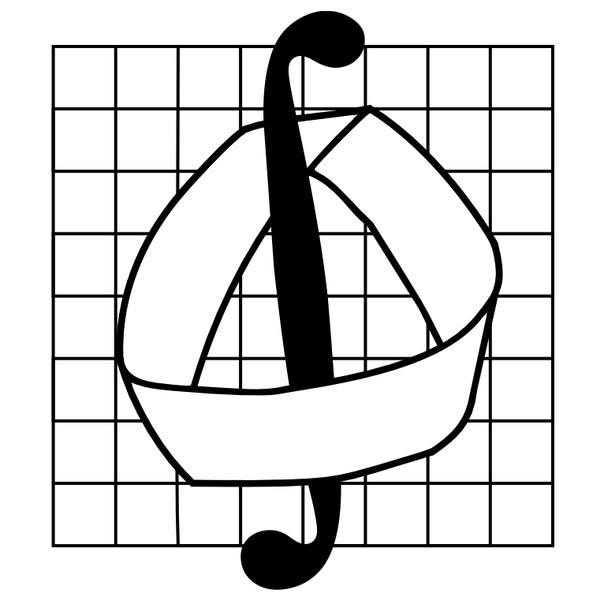
\includegraphics[width=6cm]{math_logo}
		\vspace{0.5cm}
		
		\Large
		2021
	\end{center}
\end{titlepage}
	
	\section{Условие задачи}
	\vspace{0.5cm}
	Аппроксимировать следующую задачу с помощью метода конечных элементов
	(кусочно-квадратичных) и найти решение полученной системы алгебраических 
	уравнений при различных $h$ и $f$:\\
	$$
		-(ku')' + u = f(x)
	$$
	$$
	u(0) + u'(0) = u(1) = 0,\ 
	k = \begin{cases}
			1 & x \leq 0.5\\
			\frac{3}{2} & x > 0.5
		\end{cases}
	$$
	Исследовать построенную разностную схему на устойчивость и сходимость.
	\vspace{0.5cm}
	
	\section{Решение}
	\vspace{0.5cm}
	Разобьём отрезок $\left[0,\ 1\right]$ на множество маленьких отрезков
	("конечных элементов") длиной $h$, построив на нём равномерную сетку:\\
	\begin{equation}
		\overline{D_h} = \left\{ x_j = jh,\ j = 0, \ldots, 2N-1;\ 2Nh = 1 \right\}
	\end{equation}\\
	Каждый конечный элемент образован 3 соседними узлами, всего же их $2N$.
	Будем искать приближённое решение в виде:\\
	\begin{equation}
		u^{h}(x) = \sum\limits_{j = 0}^{2N-1} c_j \cdot \varphi_j^h(x)
	\end{equation}\\
	, где $c_j$ --- неизвестные коэффициенты,\\
	, а $\left\{\varphi_j^h\right\}$ --- набор базисных функций. 
	Они имеют кусочно-квадратичный вид и представляют собой полиномы Лагранжа, 
	построенные по 3 узлам. Исходное уравнение можно записать в виде 
	$Lu = f$, где $Lu = -(ku')' + u$.\\\\
	Применяем \textbf{метод Галёркина}: 
	неизвестные коэффициенты $c_j$ определяются из условия
	ортогональности невязки базисным функциям $Ac = b$, в которой:\\
	\begin{equation}
		a_{ij} = \left( L\varphi_j^h,\ \varphi_i^h \right),\
		b_i = \left( f,\ \varphi_i^h \right);\
		i,\ j = 1,2,\ldots,N-1
	\end{equation}\\
	\begin{equation}
		\sum\limits_{j = 0}^{2N-1} c_j 
		\cdot 
		\int_{0}^{1} L\varphi_j^h \cdot \varphi_i^h dx = 
		\int_{0}^{1} f \cdot \varphi_i^h dx
	\end{equation}\\
	Кроме этих уравнений будут граничные:
	\begin{equation}
		\begin{cases}
			u(0) + u'(0) = 0\\
			u(1) = 0
		\end{cases}
	\end{equation}\\
	\begin{figure}[t]
		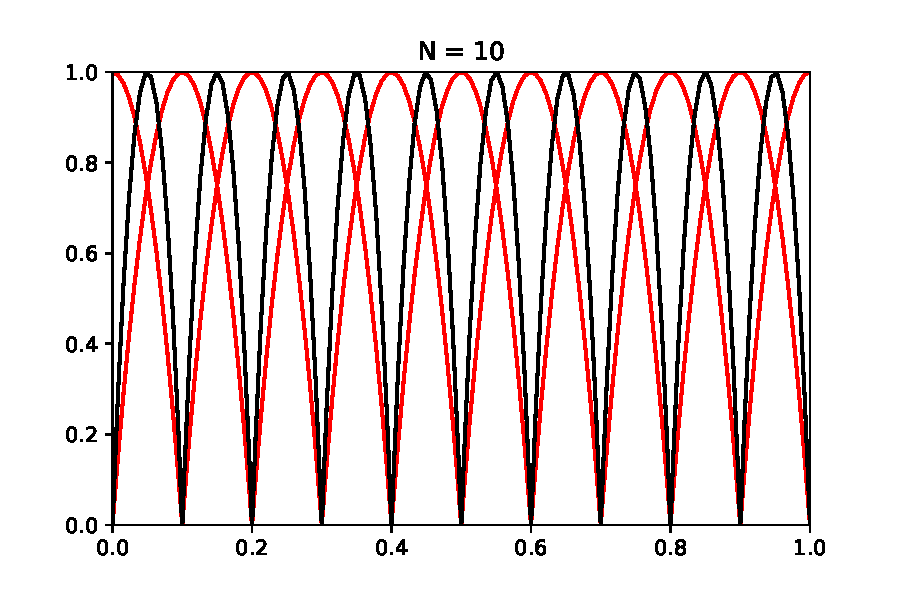
\includegraphics{basis_function}
		\caption{Базисные функции.}
		\label{ris:basis_function}
	\end{figure}
	Получим явный вид формулы для элементов матрицы $A$:\\
	\begin{multline}
		a_{ij} = \left( L\varphi_j^h,\ \varphi_i^h \right) = 
		\int_{0}^{1} L\varphi_j^h \cdot \varphi_i^h dx =
		\int_{0}^{1} -(k(x)(\varphi_j^h)')'\varphi_i^h + \varphi_j^h\varphi_i^h dx =\\
		-k(x)(\varphi_j^h)'\underbrace{\varphi_i^h}_{\text{0}}\bigg|_0^1+
		\int_{0}^{1} k(x)(\varphi_j^h)'(\varphi_i^h)' + \varphi_j^h\varphi_i^h dx
	\end{multline}\\
	Следовательно:
	\begin{equation}
		a_{ij} = \int_{0}^{1} k(x)(\varphi_j^h)'(\varphi_i^h)' + \varphi_j^h\varphi_i^h dx,\ 
		k(x) = \begin{cases}
				1 & x \leq 0.5\\
				\frac{3}{2} & x > 0.5
			\end{cases}
	\end{equation}\\
	Кусочно-квадратичные базисные функции имеют вид:\\
	\begin{equation}
		\begin{cases}
			\overline{\varphi}_j^h = \frac{(h(j-1)-x)(-h(j+1)+x)}{h^2},\ j = 0,\ldots, N\\
			\widehat{\varphi}_j^h = \frac{4(hj-x)(-h(j+1)+x)}{h^2},\ j = 0,\ldots, N
		\end{cases}
	\end{equation}\\
	Матрица $A$ выглядит так (первая строка следует из краевых условий):\\
	$$ 
	\begin{pmatrix} 
		1 & 
			\frac{4}{h} &
			\frac{2}{h} &
			0 &
			0 &
			\ldots &\\
		(L\widehat{\varphi}_0, \overline{\varphi}_0) & 
			(L\widehat{\varphi}_0, \widehat{\varphi}_0) &
			(L\widehat{\varphi}_0, \overline{\varphi}_1) &
			0 &
			0 &
			\ldots &\\
		(L\overline{\varphi}_1, \overline{\varphi}_0) & 
			(L\overline{\varphi}_1, \widehat{\varphi}_0) &
			(L\overline{\varphi}_1, \overline{\varphi}_1) &
			(L\overline{\varphi}_1, \widehat{\varphi}_1) &
			(L\overline{\varphi}_1, \overline{\varphi}_2) &
			\ldots &\\
		0 &
			0 &
			(L\widehat{\varphi}_1, \overline{\varphi}_1) &
			(L\widehat{\varphi}_1, \widehat{\varphi}_1) &
			(L\widehat{\varphi}_1, \overline{\varphi}_2) &
			\ldots &\\
		\vdots &
			\vdots &
			\vdots &
			\vdots & 
			\vdots &
			\ddots &\\ 
	\end{pmatrix} 
	$$\\
	Воспользуемся краевыми условиями, чтобы переопределить коэффициенты $a_{ij}$:\\
	$$
		u(0) + u'(0) = 0 
		\Rightarrow c_0\overline{\varphi}_0(0) + 
			(c_1\widehat{\varphi}_1(0) + c_2\overline{\varphi}_2(0))' = 0
	$$
	$$
		\Rightarrow c_1 + \frac{4}{h}c_2 + \frac{2}{h}c_3 = 0
		\Rightarrow a_{00} = 1,\ a_{01} = \frac{4}{h},\ a_{02} = \frac{2}{h},\ b_{0} = 0
	$$
	$$
		u(1) = 0 
			\Rightarrow c_{2N-1}\varphi_{2N-1} = 0 
			\Rightarrow c_{2N-1} = 0
	$$\\
	В итоге, базисные функции будут иметь вид, 
	показанный на Рис. \ref{ris:basis_function}.
	Вычислим элементы матрицы $A$ 
	(с помощью Wolfram Mathematica 12.3.0) используя явную формулу базисной функции (8), 
	явную формулу элемента матрицы (6), вид носителя базисной функции.\\
	$$
		(L\overline{\varphi}_j^h, \overline{\varphi}_j^h) =
		\int_{x_{j-1}}^{x_{j+1}} [(\overline{\varphi}_j^h)'(\overline{\varphi}_j^h)' +
		\overline{\varphi}_j^h\overline{\varphi}_j^h]dx =
		\frac{16h}{15} + \frac{8}{3h}
	$$\\
	$$
		(L\widehat{\varphi}_j^h, \widehat{\varphi}_j^h) =
		\int_{x_{j}}^{x_{j+1}} [(\widehat{\varphi}_j^h)'(\widehat{\varphi}_j^h)' +
		\widehat{\varphi}_j^h\widehat{\varphi}_j^h]dx =
		\frac{8h}{15} + \frac{16}{3h}
	$$\\
	$$
		(L\overline{\varphi}_j^h, \widehat{\varphi}_{j+1}^h) =
		\int_{x_{j}}^{x_{j+1}} [(\overline{\varphi}_j^h)'(\widehat{\varphi}_{j+1}^h)' +
		\overline{\varphi}_j^h\widehat{\varphi}_{j+1}^h]dx =
		\frac{7h}{15} + \frac{4}{3h},\ j = 2k
	$$\\
	$$
		(L\widehat{\varphi}_j^h, \overline{\varphi}_{j+2}^h) =
		\int_{x_{j}}^{x_{j+1}} [(\widehat{\varphi}_j^h)'(\overline{\varphi}_{j+2}^h)' +
		\widehat{\varphi}_j^h\overline{\varphi}_{j+2}^h]dx =
		\frac{7h}{15} + \frac{4}{3h},\ j = 2k
	$$\\
	Теперь вычислим вектор $b$:
	$$
	\overline{b}_j = (f, \overline{\varphi}_j^h) = 
		\int_{0}^{1} f\overline{\varphi}_j^h \, dx =
		\frac{4}{3} hf(hj) 
	$$
	$$
	\widehat{b}_j = (f, \widehat{\varphi}_j^h) = 
		\int_{0}^{1} f\widehat{\varphi}_j^h \, dx = 
		\frac{2}{3} hf(hj)
	$$\\
	Вектор $b$ заполняется следующим образом:
	$$
		b = (\overline{b}_{0}, \widehat{b}_0, \overline{b}_1, \widehat{b}_1, ...)
	$$
	\vspace{0.5cm}
	\newpage
	
	\section{Аппроксимация, сходимость и результаты}
	\vspace{0.5cm}
	Пусть в правой части стоит функция:\\
	$$
		f(x) := -2\pi \cos (\pi x^2) + \sin (\pi x^2) + 4 \pi^2 x^2 \sin (\pi x^2)
	$$
	Тогда аналитическим решением нашей задачи будет:\\
	$$
		U_{anal} = \sin (\pi x^2)
	$$
	\begin{figure}[h]
		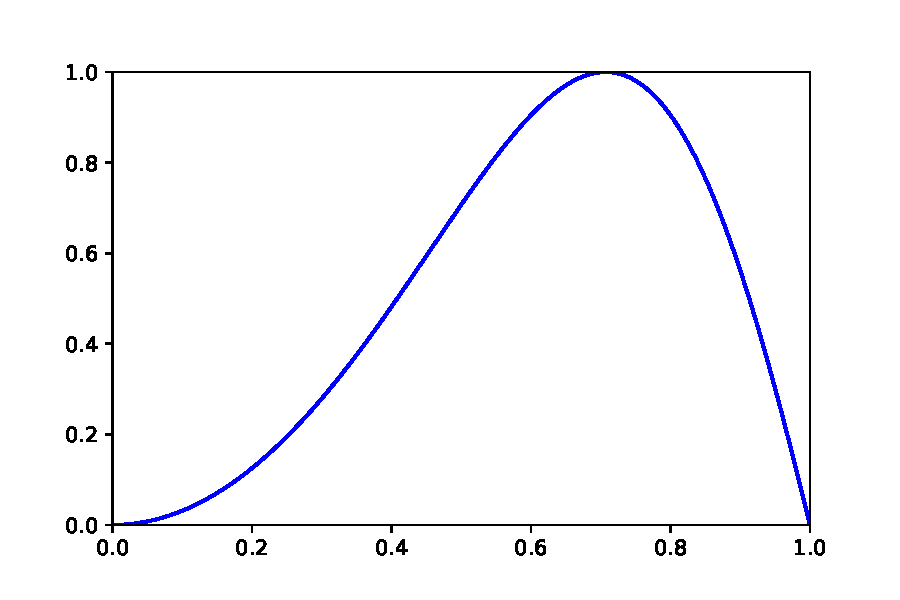
\includegraphics{anal}
		\caption{$U_{anal} = \sin (\pi x^2)$}
	\end{figure}
	
	
	\vspace{0.5cm}
	\newpage
	
	\subsection{Аппроксимация}
	\vspace{0.5cm}
	Аппроксимируем решение с данной правой частью и построим графики обеих функций для 
	$N = 5,\ 10,\ 50,\ 100,\ 500,\ 1000,\ 5000,\ 10000$.\\
	\begin{figure}[h]
		\begin{minipage}[h]{0.47\linewidth}
			\center{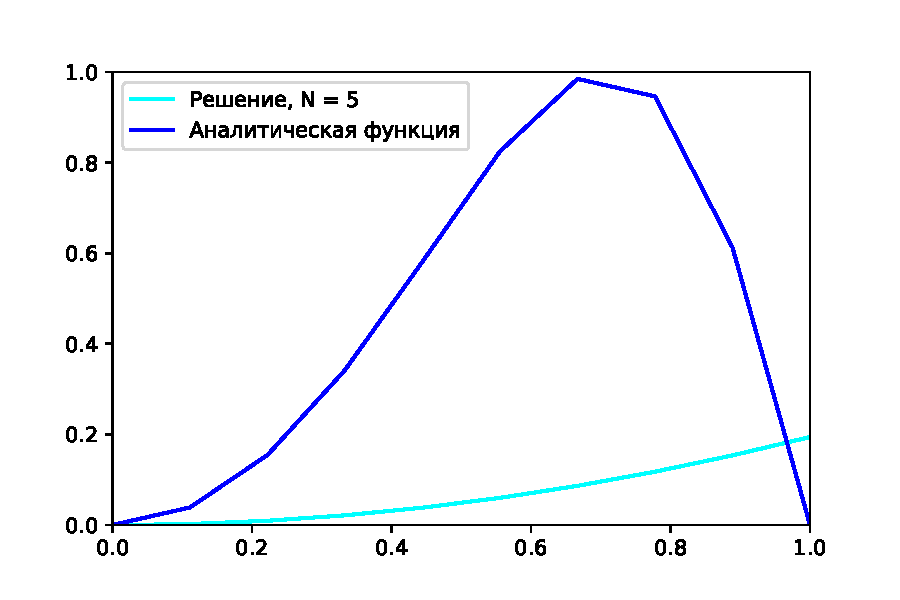
\includegraphics[width=1\linewidth]{result_N=5}}\\
		\end{minipage}
		\hfill
		\begin{minipage}[h]{0.47\linewidth}
			\center{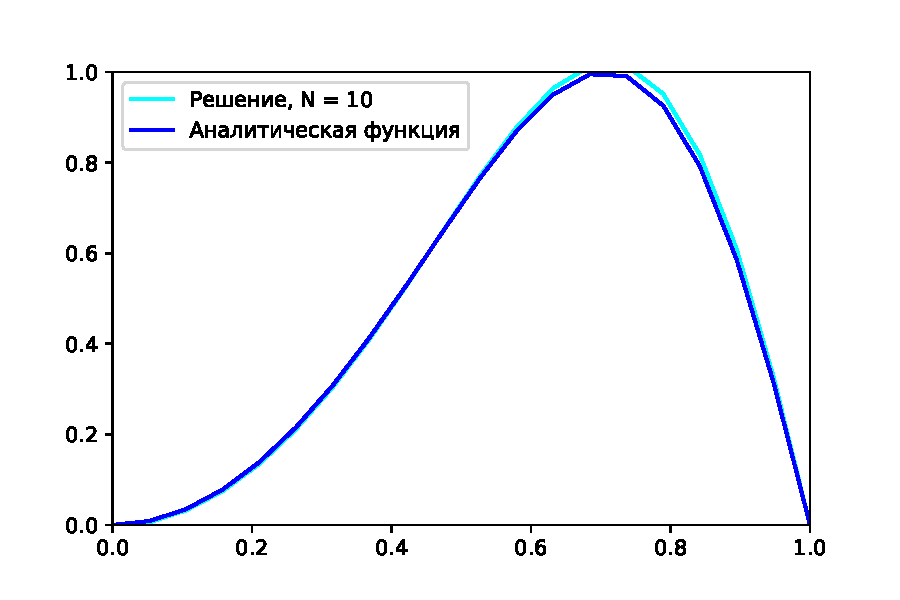
\includegraphics[width=1\linewidth]{result_N=10}}\\
		\end{minipage}
		\vfill
		\begin{minipage}[h]{0.47\linewidth}
			\center{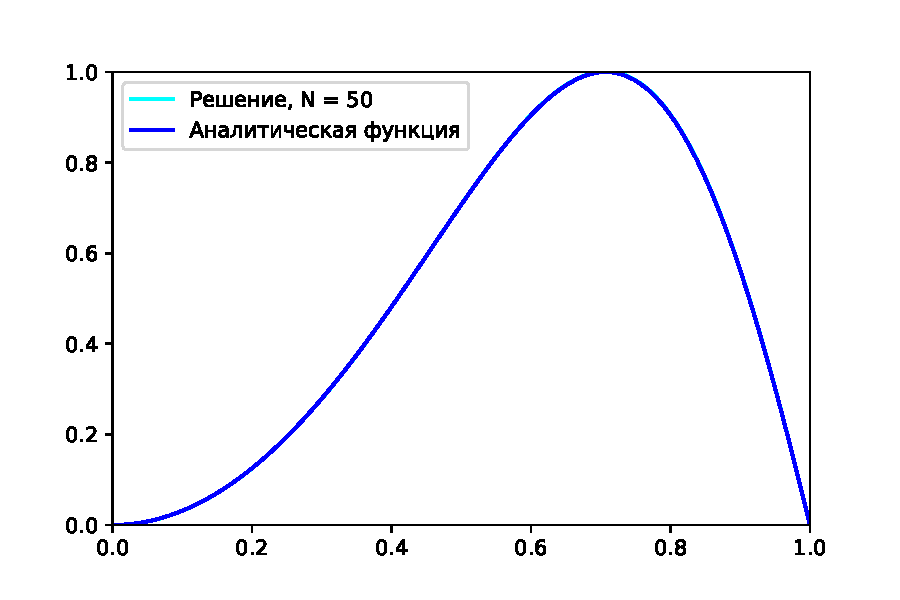
\includegraphics[width=1\linewidth]{result_N=50}}\\
		\end{minipage}
		\hfill
		\begin{minipage}[h]{0.47\linewidth}
			\center{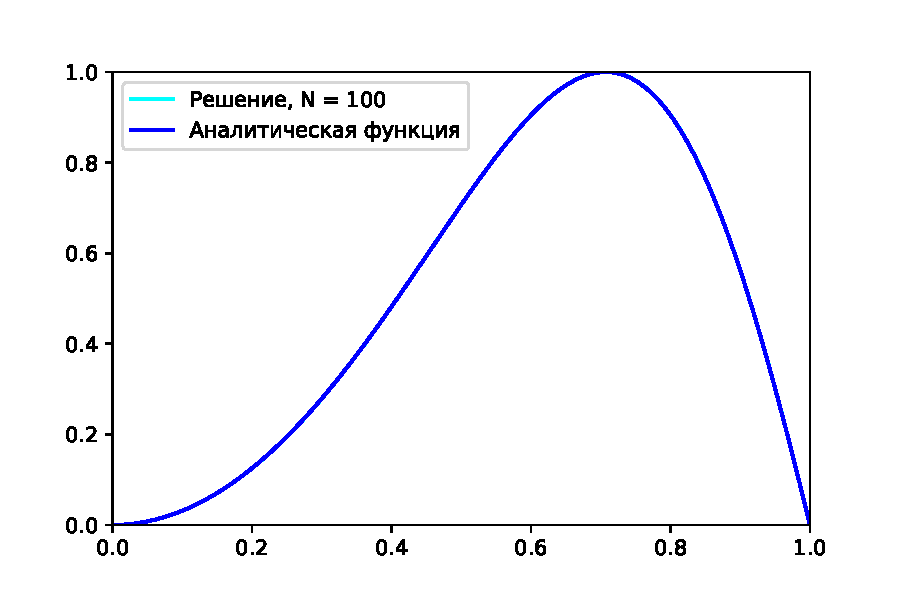
\includegraphics[width=1\linewidth]{result_N=100}}\\
		\end{minipage}
		\vfill
		\begin{minipage}[h]{0.47\linewidth}
			\center{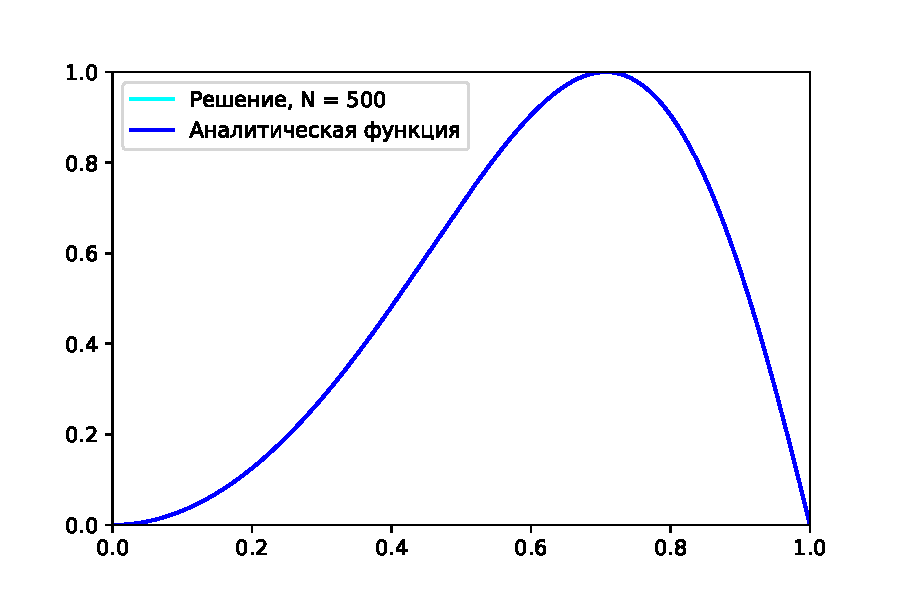
\includegraphics[width=1\linewidth]{result_N=500}}\\
		\end{minipage}
		\hfill
		\begin{minipage}[h]{0.47\linewidth}
			\center{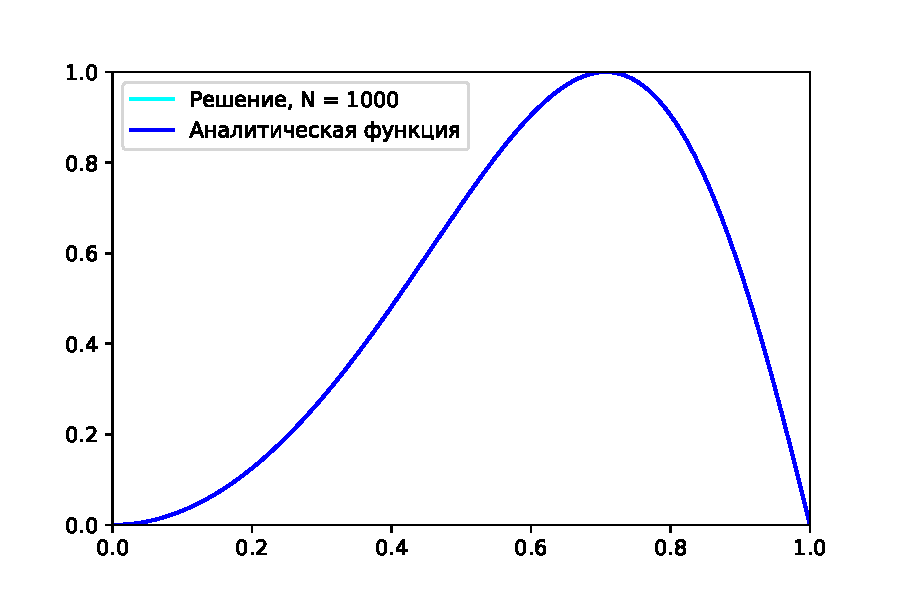
\includegraphics[width=1\linewidth]{result_N=1000}}\\
		\end{minipage}
		\vfill
		\begin{minipage}[h]{0.47\linewidth}
			\center{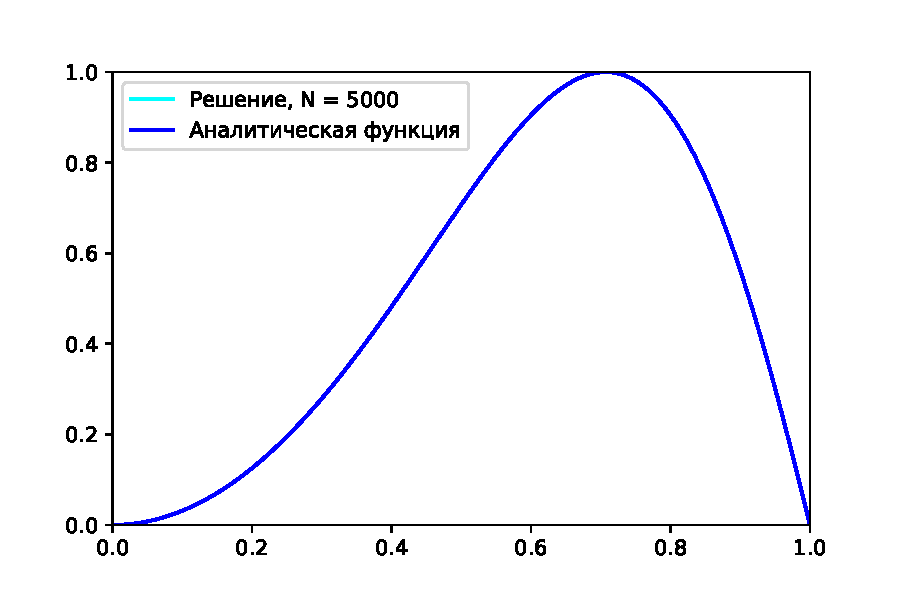
\includegraphics[width=1\linewidth]{result_N=5000}}\\
		\end{minipage}
		\hfill
		\begin{minipage}[h]{0.47\linewidth}
			\center{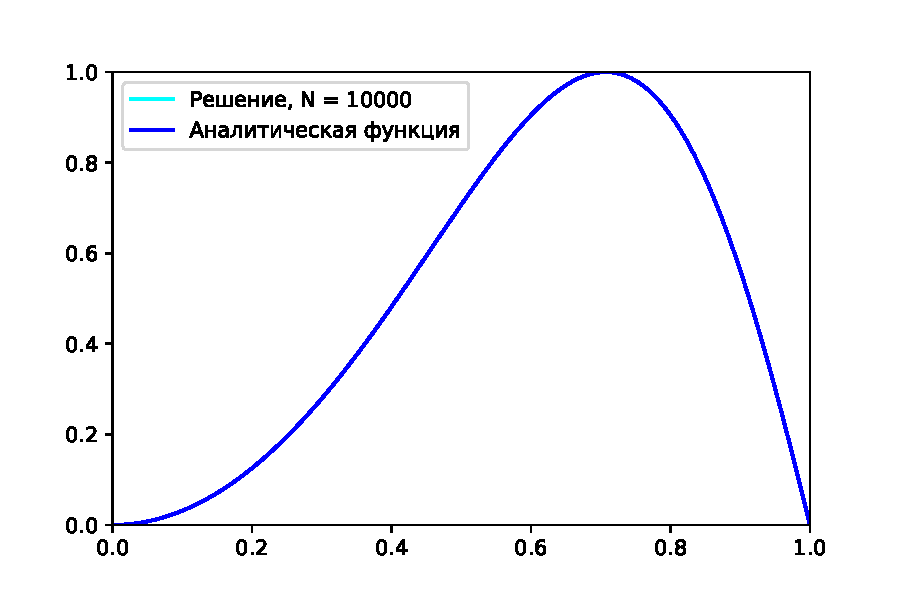
\includegraphics[width=1\linewidth]{result_N=10000}}\\
		\end{minipage}
	\end{figure}
	\vspace{0.5cm}
	\newpage
	
	\subsection{Погрешность}
	\vspace{0.5cm}
	Погрешность $\delta = max_{x \in [0,1]} |u_{analytical} - u_{approximation}|$ 
	при различных N = 5,\ 10,\ 50,\ 100,\ 500,\ 1000,\ 5000,\ 10000 
	соответственно равна:\\
	\begin{table}[h]
	\centering
		\begin{tabular}{ll}
		\hline
		N & Погрешность \\
		\hline
		5 & 9.12989e-02\\
		10 & 2.59366e-02\\
		50 & 1.10012e-03\\
		100 & 2.75474e-04\\
		500 & 1.10292e-05\\
		1000 & 2.75746e-06\\
		5000 & 1.10415e-07\\
		10000 & 2.70430e-08\\
		\hline
		\end{tabular}
	\end{table}\\
	\begin{figure}[h]
		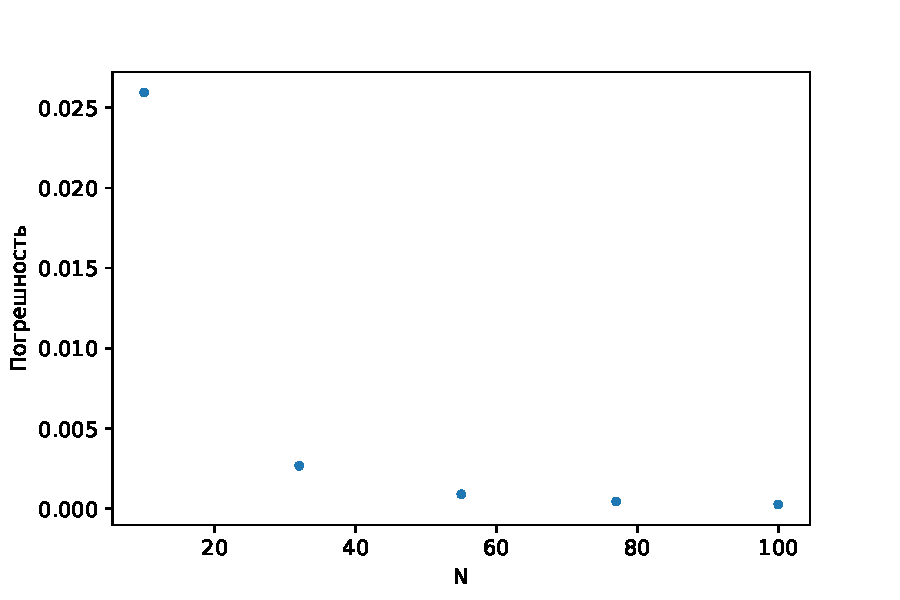
\includegraphics{norm}
		\caption{Погрешность}
	\end{figure}
\end{document}